%! Author = Philipp Emmenegger
%! Date = 10/06/2021

\section{Multithreading Grundlagen}
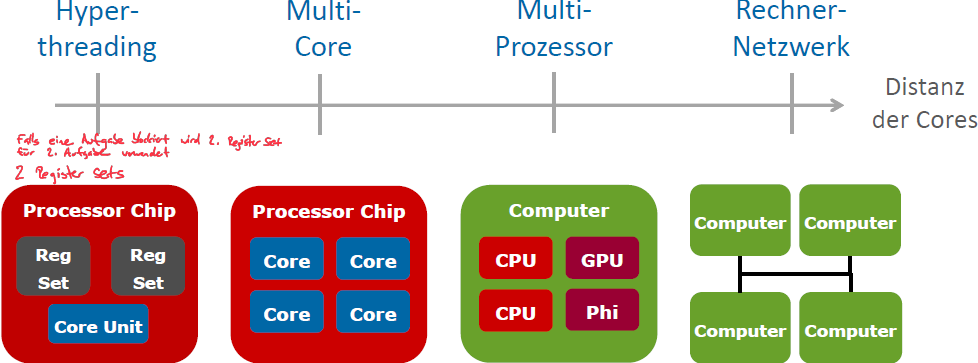
\includegraphics[width=\linewidth]{img/stufen.png}
\textbf{Parallelität:} Aufteilung in Teilabläufe, laufen gleichzeitig auf mehreren Prozessoren.
\textbf{Nebenläufigkeit:} Gleichzeitig oder verzahnt ausführbare Abläufe, greifen au gemeinsame Ressourcen zu.
\textbf{Prozess:} Parallel laufende Programm-Instanz im System. Eigener Adressraum.
\textbf{Thread:} Parallele Ablaufsequenz innerhalb eines Programms. Teilen gleichen Adressraum.

\subsection{Thread-Implementationen}
\textbf{User-Level Threads:} Im Prozess implementiert.
Keine echte Parallelität durch mehrere Prozessoren.
\textbf{Kernel-Level Threads:} Im Kernel implementiert (Multi-Core Ausnutzung).
Kontextwechsel vom Prozess per SW-Interrupt.
\textbf{Thread Scheduling:} Processor Sharing - \#Threads \textgreater \#Prozessoren.

\subsection{Prozessor Multiplexing}
\textbf{Verzahnte Ausführung:} Instruktionen von mehreren Threads in Teilsequenzen. Illusion der Parallelität.
\textbf{Kontextwechsel:} \textit{Synchron} (Freiwillige abgabe), Thread wechselt zu wait. \textit{Asynchron:} (gezwungene Abgabe) Begrenzte Laufzeit für Threads.

\subsection{Multi-Tasking:}
\textbf{Kooperativ:} Threads initiieren Kontextwechsel synchron (freiwillig). Scheduler kann Thread nicht unterbrechen.
\textbf{Preemtiv:} Scheduler kann Thread mit Timer-Interrupt asynchron unterbrechen (Time-Sliced-Scheduling)(\textit{Standart heute}).
\textbf{Thread Zustände:} Ready, Waiting, Running.

\subsection{Multi-Thread Programmierung}
\subsubsection{JVM Thread Modell}
Java ist ein Single Process System. 
JVM ist ein Prozess im Bsys.
\textbf{Main-Thread} wird beim Aufstarten der JVM anhand \textit{main()} Methode erzeugt.
JVM läuft, solange Threads laufen (Ausnahme Daemon Threads).
\begin{lstlisting}
var myThread = new Thread(() -> { // ... });
myThread.start();
\end{lstlisting}
Thread wird erst bei \textit{start()} erzeugt. Führt \textit{run()}-Methode des Runnable Interface aus.
Thread endet beim Verlassen von \textit{run()}.\\
\textbf{Nicht-Determinismus:} Threads laufen ohne Vorkehrungen beliebig verzahnt oder parallel.
\subsubsection{Explizite Runnable-Implementation:}
\begin{lstlisting}
class SimpleLogic implements Runnable {
    @Override
    public void run() { // ... }
}
var myThread = new Thread(new SimpleLogic()).start();
\end{lstlisting}

\subsubsection{Sub-Klasse von Thread}
\begin{lstlisting}
class SimpleThread extends Thread {
    @Override 
    public void run() { // ... }
}
var myThread = new SimpleThread().start();
\end{lstlisting}

\subsubsection{Thread Join}
Warten auf Beendigung eines Threads. \textit{t2.join()} blockiert, solange t2 läuft.

\subsubsection{Thread Passivierung}
\textbf{Thraed.sleep(ms):} Laufender Thread geht in Wartezustand, dann ready.
\textbf{Thread.yield():} Gibt Prozesor frei, direkt ready.